\documentclass[10pt,a4paper]{article}
\usepackage[utf8]{inputenc}
\usepackage[margin=0.6in]{geometry}
\usepackage{graphicx}
\usepackage{microtype}
\usepackage{titlesec}
\usepackage{hyperref}
\usepackage{booktabs}
\usepackage{enumitem}
\usepackage{xcolor}
\usepackage{tabularx}

\graphicspath{{certificates/}{./}}

\definecolor{amritablue}{RGB}{0, 51, 102}
\definecolor{darkgray}{RGB}{50, 50, 50}

\hypersetup{
    colorlinks=true,
    linkcolor=amritablue,
    urlcolor=amritablue,
}

\titlespacing*{\section}{0pt}{4pt}{2pt}
\titlespacing*{\subsection}{0pt}{3pt}{1pt}

\titleformat{\section}
  {\normalfont\small\bfseries\color{amritablue}\uppercase}
  {\thesection}{1em}{}[\titlerule]

\setlist{nosep, leftmargin=13pt}

\begin{document}
\pagestyle{empty}

% =========================================================
% PAGE 1: COURSE COMPLETION CERTIFICATE
% =========================================================
\begin{center}
    {\large\textbf{\color{amritablue}AMRITA VISHWA VIDYAPEETHAM}}\\[1pt]
    {\footnotesize\textbf{Amrita School of Computing, Coimbatore --- Department of Computer Science and Engineering}}\\[2pt]
    {\footnotesize\textbf{Technical Enrichment Activity: Professional Online Certification (20 Marks)}}\\[1pt]
    {\scriptsize Official Course Completion Certificate}
\end{center}

\vspace{-4pt}
\hrule height 0.8pt
\vspace{6pt}

\noindent
\begin{tabularx}{\textwidth}{@{}l X l X@{}}
    \textbf{Student Name:} & Edavalapati Aashiq & \textbf{Course Title:} & Software Defined Networking \\
    \textbf{Roll Number:} & CB.SC.U4CSE23560 & \textbf{Platform / Provider:} & Coursera / The University of Chicago \\
    \textbf{Degree \& Branch:} & B.Tech CSE (VII Semester) & \textbf{Project Guide:} & Ms. Neethu M R (Asst. Professor) \\
\end{tabularx}

\vspace{12pt}
\begin{center}
    \fbox{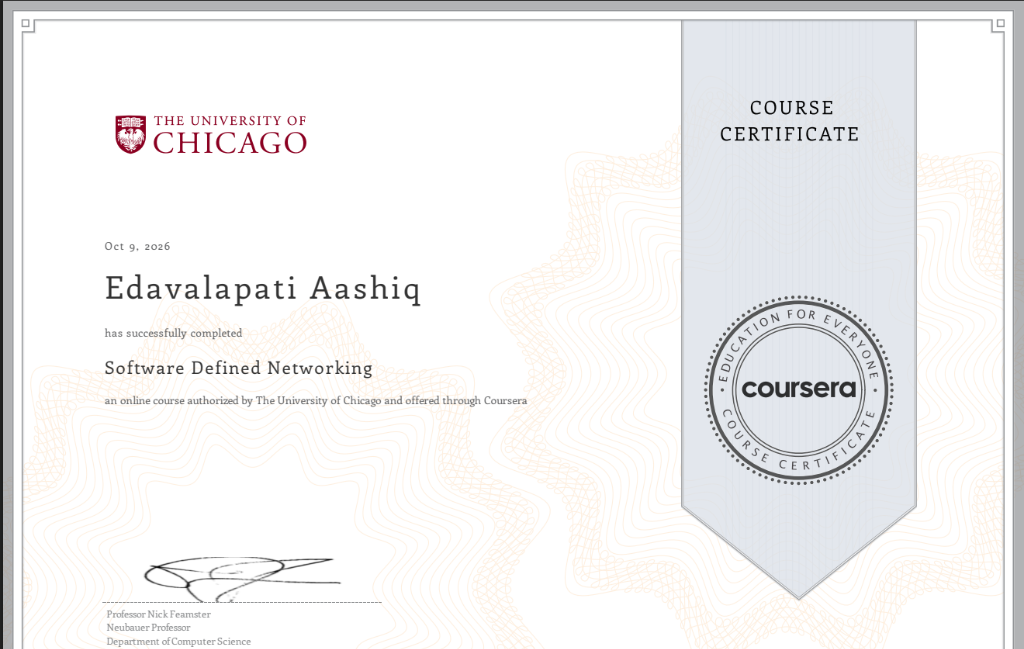
\includegraphics[width=0.96\textwidth, height=0.70\textheight, keepaspectratio]{aashiq_cert.png}}
\end{center}

\vfill
\begin{center}
    {\footnotesize\textbf{Credential Verification URL:} \url{https://coursera.org/share/e6df331f2250afa69a53ec4b051f1f01}}
\end{center}

\clearpage

% =========================================================
% PAGE 2: TECHNICAL ALIGNMENT REPORT
% =========================================================
\begin{center}
    {\large\textbf{\color{amritablue}AMRITA VISHWA VIDYAPEETHAM}}\\[1pt]
    {\footnotesize\textbf{Amrita School of Computing, Coimbatore --- Department of Computer Science and Engineering}}\\[2pt]
    {\footnotesize\textbf{Technical Enrichment Activity: Professional Online Certification (20 Marks)}}\\[1pt]
    {\scriptsize Course Completion Details \& One-Page Technical Alignment Report}
\end{center}

\vspace{-4pt}
\hrule height 0.8pt
\vspace{4pt}

\noindent
\begin{tabularx}{\textwidth}{@{}l X l X@{}}
    \textbf{Student Name:} & Edavalapati Aashiq & \textbf{Course Title:} & Software Defined Networking \\
    \textbf{Roll Number:} & CB.SC.U4CSE23560 & \textbf{Platform / Provider:} & Coursera / The University of Chicago \\
    \textbf{Degree \& Branch:} & B.Tech CSE (VII Semester) & \textbf{Duration / Effort:} & 15--20 Hours (10--20 Hour Category) \\
    \textbf{Project Guide:} & Ms. Neethu M R (Asst. Professor) & \textbf{Verification URL:} & \url{https://coursera.org/share/e6df331f2250afa69a53ec4b051f1f01} \\
\end{tabularx}

\vspace{3pt}
\noindent
\textbf{B.Tech Project Title:} \textit{EdgeTrust-VANET: A Decentralized Trust Management and Machine Learning Framework for Secure Vehicular Ad Hoc Networks}

\vspace{2pt}
\section*{1. Course Curriculum \& Technical Competencies Acquired}
The advanced certification \textit{Software Defined Networking} (The University of Chicago via Coursera) teaches architectural principles, abstractions, and programming paradigms for modern software-driven network control:
\begin{itemize}
    \item \textbf{Control-Data Plane Disaggregation:} Architectural separation of forwarding hardware (data plane) from centralized network intelligence (control plane).
    \item \textbf{OpenFlow Protocol \& Flow Table Programming:} Designing flow matches, actions, packet-in/packet-out event handling, and pipeline processing.
    \item \textbf{Network Virtualization \& Programmable Routing:} Dynamic topology mapping, shortest-path calculation with custom link penalties, and policy-based traffic steering.
    \item \textbf{Centralized Security Enforcement:} Network-wide anomaly isolation, rapid revocation broadcast, and mitigation of distributed denial-of-service (DoS) attacks.
\end{itemize}

\section*{2. Technical Justification: How the Course Directly Supports EdgeTrust-VANET}
In EdgeTrust-VANET, static hop-by-hop ad-hoc routing fails under insider attacks and high vehicle mobility. The Software-Defined Vehicular Network (SDVN) principles acquired in this course directly enabled the design of our **Tier 4 Centralized SDN Controller** and global security orchestration:

\begin{enumerate}
    \item \textbf{Hierarchical SDVN Architecture Formulation (Tier 4 Controller):} 
    Applying the control-plane decoupling paradigms taught by Prof. Feamster, we designed Tier 4 as a centralized SDN controller that maintains a global network graph and coordinates Regional Fog nodes (Tier 3) and Roadside Units (Tier 2) over a 10~Gbps high-bandwidth optical fiber backbone.

    \item \textbf{Trust-Penalized Dynamic Routing Algorithm:} 
    Standard routing algorithms optimize purely for physical distance, blindly traversing malicious intermediate nodes. Applying SDN programmable path computation, we engineered a trust-weighted Dijkstra algorithm where edge cost is scaled inversely by node reputation:
    \[
    C_{ij} = \frac{d_{ij}}{T_i \cdot T_j}
    \]
    This dynamically steers critical vehicular multi-hop traffic around degraded nodes ($0.40 \le T < 0.70$) without requiring protocol-level reconfiguration on individual vehicles.

    \item \textbf{OpenFlow Flow Table Synchronization \& Dynamic CRL Revocation:} 
    Using the OpenFlow abstractions covered in the course, our SDN controller dynamically pushes proactive flow modifications to RSUs upon detecting malicious actors ($T < 0.40$). This automates instantaneous Certificate Revocation List (CRL) distribution, blacklisting attacker MACs across the entire urban corridor.

    \item \textbf{Low-Latency Inter-RSU Fiber Ring Coordination:} 
    The course's traffic engineering and state synchronization principles guided our design of the $<1$~ms local fiber ring connecting edge RSUs, guaranteeing seamless handover of vehicle reputation tokens without security context loss.
\end{enumerate}

\section*{3. Measurable Project Outcomes Supported by this Certification}
\noindent
\begin{tabularx}{\textwidth}{@{}X X X@{}}
    \textbf{Architecture Design:} Tier 4 SDN Controller Orchestration & 
    \textbf{Routing Optimization:} Trust-Dijkstra Path Penalty & 
    \textbf{Academic Status:} IEEE Conference Paper Under Review \\
\end{tabularx}

\end{document}
